\pdfoutput=1
\documentclass{article}


% alptex + small aesthetic tweaks + some extra math defs
%\RequirePackage[l2tabu, orthodox]{nag}

% FONTS
\usepackage[utf8]{inputenc} % allow utf-8 input
\usepackage[T1]{fontenc}    % use 8-bit T1 fonts

% Replace default Latin Modern typewriter with its proportional counterpart
% http://www.tug.dk/FontCatalogue/lmoderntypewriterprop/
\renewcommand*\ttdefault{lmvtt}


%%% OPTION 1 - Fourier Math + New Century Schoolbook + ParaType Sans

% % Import Fourier Math (this imposes its own New Century Schoolbook type)
% % http://www.ctan.org/tex-archive/fonts/fouriernc/
% \usepackage{fouriernc}
% \usepackage{amsmath}
% % Replace with TeX Gyre Schola version of New Century Schoolbook (must scale!)
% % http://www.tug.dk/FontCatalogue/tgschola/
% \usepackage[scale=0.92]{tgschola}
% \usepackage[scaled=0.88]{PTSans}

%% OPTION 2 - MathDesign Math + Bitstream Charter + ParaType Sans

% Import MathDesign (this brings along Bitstream Charter)
% http://www.ctan.org/tex-archive/fonts/mathdesign/
\usepackage[bitstream-charter]{mathdesign}
\usepackage{amsmath}
\usepackage[scaled=0.92]{PTSans}


% %%% OPTION 3 - MTPRO 2 Math + Termes Times + ParaType Sans

% \usepackage{tgtermes}
% \usepackage{amsmath}
% \usepackage[subscriptcorrection,
%             amssymbols,
%             mtpbb,
%             mtpcal,
%             nofontinfo  % suppresses all warnings
%            ]{mtpro2}
% \usepackage{scalefnt,letltxmacro}
% \LetLtxMacro{\oldtextsc}{\textsc}
% \renewcommand{\textsc}[1]{\oldtextsc{\scalefont{1.10}#1}}
% \usepackage[scaled=0.92]{PTSans}

% GEOMETRY
\usepackage[
  paper  = letterpaper,
  left   = 1.65in,
  right  = 1.65in,
  top    = 1.0in,
  bottom = 1.0in,
  ]{geometry}

% COLOR
\usepackage[usenames,dvipsnames,table]{xcolor}
%\usepackage[usenames,table]{xcolor}
\definecolor{shadecolor}{gray}{0.9}

% SPACING and TEXT
\usepackage[final,expansion=alltext]{microtype}
\usepackage[english]{babel}
\usepackage[parfill]{parskip}
\usepackage{afterpage}
\usepackage{framed}

%redefine the leftbar environment to accept a width and coloring options
\renewenvironment{leftbar}[1][\hsize]
{%
  \def\FrameCommand
  {%
    {\color{Gray}\vrule width 3pt}%
    \hspace{10pt}%
    %\hspace{0pt}\fboxsep=\FrameSep\colorbox{black!10}%
  }%
  \MakeFramed{\hsize#1\advance\hsize-\width\FrameRestore}%
}%
{\endMakeFramed}

% define a paragraph header function
\DeclareRobustCommand{\parhead}[1]{\textbf{#1}~}

% EDITING
% line numbering in left margin
\usepackage{lineno}
\renewcommand\linenumberfont{\normalfont
                             \footnotesize
                             \sffamily
                             \color{SkyBlue}}
% ragged paragraphs in right margin
\usepackage{ragged2e}
\DeclareRobustCommand{\sidenote}[1]{\marginpar{
                                    \RaggedRight
                                    \textcolor{Plum}{\textsf{#1}}}}
% paragraph counter in right margin
\newcommand{\parnum}{\bfseries\P\arabic{parcount}}
\newcounter{parcount}
\newcommand\p{%
    \stepcounter{parcount}%
    \leavevmode\marginpar[\hfill\parnum]{\parnum}%
}
% paragraph helper
\DeclareRobustCommand{\PP}{\textcolor{Plum}{\P} }

% COUNTERS
\renewcommand{\labelenumi}{\color{black!67}{\arabic{enumi}.}}
\renewcommand{\labelenumii}{{\color{black!67}(\alph{enumii})}}
\renewcommand{\labelitemi}{{\color{black!67}\textbullet}}

% FIGURES
\usepackage{graphicx}
\usepackage{wrapfig}
\usepackage[labelfont=bf,font=footnotesize,width=.9\textwidth]{caption}
\usepackage[format=hang]{subcaption}

% TABLES
\usepackage{booktabs,multirow,multicol}       % professional-quality tables

% ALGORITHMS
\usepackage[algoruled]{algorithm2e}
\usepackage{listings}
\usepackage{fancyvrb}
\fvset{fontsize=\normalsize}

% BIBLIOGRAPHY
%\usepackage{natbib}

% HYPERREF
\usepackage[colorlinks,linktoc=all]{hyperref}
\usepackage[all]{hypcap}
\hypersetup{citecolor=MidnightBlue}
\hypersetup{linkcolor=MidnightBlue}
\hypersetup{urlcolor=MidnightBlue}

% CLEVEREF must come after HYPERREF
\usepackage[nameinlink]{cleveref}

% ACRONYMS
\usepackage[acronym,smallcaps,nowarn]{glossaries}
% \makeglossaries

% COLOR DEFINITIONS
\newcommand{\red}[1]{\textcolor{BrickRed}{#1}}
\newcommand{\orange}[1]{\textcolor{BurntOrange}{#1}}
\newcommand{\green}[1]{\textcolor{OliveGreen}{#1}}
\newcommand{\blue}[1]{\textcolor{MidnightBlue}{#1}}
\newcommand{\gray}[1]{\textcolor{black!60}{#1}}

% LISTINGS DEFINTIONS
\lstdefinestyle{mystyle}{
    commentstyle=\color{OliveGreen},
    keywordstyle=\color{BurntOrange},
    numberstyle=\tiny\color{black!60},
    stringstyle=\color{MidnightBlue},
    basicstyle=\ttfamily,
    breakatwhitespace=false,
    breaklines=true,
    captionpos=b,
    keepspaces=true,
    numbers=left,
    numbersep=5pt,
    showspaces=false,
    showstringspaces=false,
    showtabs=false,
    tabsize=2
}
\lstset{style=mystyle}

% !TEX root = main.tex


\usepackage{centernot}
\usepackage{amsthm}
\usepackage{amsfonts}       % blackboard math symbols
\usepackage{nicefrac}       % compact symbols for 1/2, etc.
\usepackage{mathtools}
\usepackage{amsbsy}
\usepackage{amstext}
\usepackage{amsthm}
%\usepackage{amssymb}
\usepackage{thmtools}
\usepackage{thm-restate}

% compatibility w/ parskip https://tex.stackexchange.com/questions/25346/wrong-spacing-before-theorem-environment-amsthm
\begingroup
    \makeatletter
    \@for\theoremstyle:=definition,remark,plain\do{%
        \expandafter\g@addto@macro\csname th@\theoremstyle\endcsname{%
            \addtolength\thm@preskip\parskip
            }%
        }
\endgroup

\DeclareRobustCommand{\mb}[1]{\ensuremath{\mathbf{\boldsymbol{#1}}}}
% \DeclareRobustCommand{\mb}[1]{\mathbold{#1}}

\DeclareRobustCommand{\KL}[2]{\ensuremath{\textrm{KL}\left(#1\;\|\;#2\right)}}

% \DeclareMathOperator*{\argmax}{arg\,max}
% \DeclareMathOperator*{\argmin}{arg\,min}

\crefname{lemma}{lemma}{lemmas}
\Crefname{lemma}{Lemma}{Lemmas}
\crefname{thm}{theorem}{theorems}
\Crefname{thm}{Theorem}{Theorems}
\crefname{prop}{proposition}{propositions}
\Crefname{prop}{Proposition}{Propositions}
\crefname{assumption}{assumption}{assumptions}
\crefname{assumption}{Assumption}{Assumptions}


% \newtheorem{thm}{Theorem} % reset theorem numbering for each chapter
% \newtheorem{defn}{Definition} % definition numbers are dependent on theorem numbers
% \newtheorem{prop}[thm]{Proposition}
% \newtheorem{exmp}[thm]{Example} % same for example numbers
% \newtheorem{lemma}[thm]{Lemma}
% \newtheorem{assumption}{Assumption}
\newtheorem{corollary}[thm]{Corollary}
\newcommand\independent{\protect\mathpalette{\protect\independenT}{\perp}}
\def\independenT#1#2{\mathrel{\rlap{$#1#2$}\mkern2mu{#1#2}}}

\newcommand{\grad}{\nabla}

\renewcommand{\mid}{~\vert~}
\newcommand{\prm}{\:;\:}

\newcommand{\mbw}{\mb{w}}
\newcommand{\mbW}{\mb{W}}

\newcommand{\mbx}{\mb{x}}
\newcommand{\mbX}{\mb{X}}

\newcommand{\mby}{\mb{y}}
\newcommand{\mbY}{\mb{Y}}

\newcommand{\mbz}{\mb{z}}
\newcommand{\mbZ}{\mb{Z}}
\newcommand{\mbT}{\mb{T}}
\newcommand{\mbA}{\mb{A}}
\newcommand{\mba}{\mb{a}}

\newcommand{\mbI}{\mb{I}}
\newcommand{\mbone}{\mb{1}}

\newcommand{\mbL}{\mb{L}}

\newcommand{\mbtheta}{\mb{\theta}}
\newcommand{\mbTheta}{\mb{\Theta}}
\newcommand{\mbomega}{\mb{\omega}}
\newcommand{\mbOmega}{\mb{\Omega}}
\newcommand{\mbsigma}{\mb{\sigma}}
\newcommand{\mbSigma}{\mb{\Sigma}}
\newcommand{\mbphi}{\mb{\phi}}
\newcommand{\mbPhi}{\mb{\Phi}}

\newcommand{\mbalpha}{\mb{\alpha}}
\newcommand{\mbbeta}{\mb{\beta}}
\newcommand{\mbgamma}{\mb{\gamma}}
\newcommand{\mbeta}{\mb{\eta}}
\newcommand{\mbmu}{\mb{\mu}}
\newcommand{\mbrho}{\mb{\rho}}
\newcommand{\mblambda}{\mb{\lambda}}
\newcommand{\mbzeta}{\mb{\zeta}}

\newcommand\dif{\mathop{}\!\mathrm{d}}
\newcommand{\diag}{\textrm{diag}}
\newcommand{\supp}{\textrm{supp}}

\newcommand{\V}{\mathbb{V}}
\newcommand{\bbH}{\mathbb{H}}

\newcommand{\bbN}{\mathbb{N}}
\newcommand{\bbZ}{\mathbb{Z}}
\newcommand{\bbR}{\mathbb{R}}
\newcommand{\bbS}{\mathbb{S}}

\newcommand{\cL}{\mathcal{L}}
\newcommand{\cD}{\mathcal{D}}

\newcommand{\cN}{\mathcal{N}}
\newcommand{\cT}{\mathcal{T}}
\newcommand{\Gam}{\textrm{Gam}}
\newcommand{\InvGam}{\textrm{InvGam}}

% \newcommand{\qedsymbol}{\rule{0.7em}{0.7em}}

\newcommand{\g}{\, | \,}
\newcommand{\s}{\, ; \,}

\newcommand{\indpt}{\protect\mathpalette{\protect\independenT}{\perp}}
\newcommand{\E}[2]{\mathbb{E}_{#1}\left[#2\right]}

\def\checkmark{\tikz\fill[scale=0.4](0,.35) -- (.25,0) -- (1,.7) -- (.25,.15) -- cycle;} 


\usepackage{booktabs,arydshln}
\makeatletter
\def\adl@drawiv#1#2#3{%
        \hskip.5\tabcolsep
        \xleaders#3{#2.5\@tempdimb #1{1}#2.5\@tempdimb}%
                #2\z@ plus1fil minus1fil\relax
        \hskip.5\tabcolsep}
\newcommand{\cdashlinelr}[1]{%
  \noalign{\vskip\aboverulesep
           \global\let\@dashdrawstore\adl@draw
           \global\let\adl@draw\adl@drawiv}
  \cdashline{#1}
  \noalign{\global\let\adl@draw\@dashdrawstore
           \vskip\belowrulesep}}
\makeatother

\newenvironment{proofsk}{%
  \renewcommand{\proofname}{Proof sketch}\proof}{\endproof}

\renewcommand{\epsilon}{\varepsilon}

%********************************************************************
% Extra theorem environments
%********************************************************************

\declaretheorem[style=plain,name=Theorem]{theorem}
\declaretheorem[style=plain,sibling=theorem,name=Lemma]{lemma}
\declaretheorem[style=plain,sibling=theorem,name=Proposition]{proposition}
\declaretheorem[style=plain,sibling=theorem,name=Corollary]{cor}
\declaretheorem[style=plain,sibling=theorem,name=Claim]{claim}
\declaretheorem[style=plain,sibling=theorem,name=Conjecture]{conj}
\declaretheorem[style=definition,sibling=theorem,name=Definition]{defn}
\declaretheorem[style=definition,name=Assumption]{assumption}
\declaretheorem[style=definition,sibling=theorem,name=Example]{example}
\declaretheorem[style=remark,sibling=theorem,name=Remark]{remark}

\newenvironment{example*}
 {\pushQED{\qed}\example}
 {\popQED\endexample}
\numberwithin{equation}{section}

% This file contains definitions of custom macros
% ------------------------------------------------------------------------------

\newcommand{\defnphrase}[1]{\emph{#1}}

\global\long\def\floor#1{\lfloor#1\rfloor}

%\newcommand{\st}{\,:\,}
\newcommand{\defeq}{\coloneqq}
\newcommand{\asympeq}{\ \sim\ }

\newcommand{\Reals}{\mathbb{R}}
\newcommand{\Nats}{\mathbb{N}}
\newcommand{\NNReals}{\Reals_{+}}


\newcommand{\exclude}{\backslash}

\newcommand{\eps}{\varepsilon}

\renewcommand{\Re}{\mathrm{Re}}
\renewcommand{\Im}{\mathrm{Im}}

\DeclareMathOperator*{\argmin}{argmin}
\DeclareMathOperator*{\argmax}{argmax}
\DeclareMathOperator*{\logit}{logit}


% Graph theory
\newcommand{\edges}{e}
\newcommand{\vertices}{v}
\newcommand{\loops}{l}


% Probability
\newcommand{\EE}{\mathbb{E}}
\newcommand{\var}{\mathrm{var}}
\renewcommand{\Pr}{\mathrm{P}}
\newcommand{\convPr}{\xrightarrow{\,p\,}}
\newcommand{\convDist}{\xrightarrow{\,d\,}}
\newcommand{\equaldist}{\overset{d}{=}}
\newcommand{\upto}{\!\uparrow\!}
\newcommand{\given}{\mid}
\newcommand{\as}{\textrm{ a.s.}}
\newcommand{\equalas}{\overset{\mathrm{a.s.}}{=}}
\newcommand{\abs}[1]{\left\lvert#1 \right\rvert}
\newcommand{\intd}{\mathrm{d}}
\newcommand{\dist}{\ \sim\ }
\newcommand{\distiid}{\overset{\mathrm{iid}}{\dist}}
\newcommand{\distind}{\overset{ind}{\dist}}
\newcommand{\dtv}[1]{\|#1\|_{\mathrm{TV}}}
%\newcommand{\PP}{\Pi}
\newcommand{\PPDist}{\mathrm{PP}}

\newcommand{\Lebesgue}{\Lambda}
\newcommand{\NatSubs}[1]{\tilde \Nats_{#1}}

% Causality
\newcommand{\cdo}{\mathrm{do}} 

% Distributions
\newcommand{\normalDist}{\mathrm{Normal}}
\newcommand{\diriDist}{\mathrm{Diri}}
\newcommand{\categDist}{\mathrm{Cat}}
\newcommand{\betaDist}{\mathrm{Beta}}
\newcommand{\bernDist}{\mathrm{Bern}}
\newcommand{\binDist}{\mathrm{Bin}}
\newcommand{\uniDist}{\mathrm{Uni}}
\newcommand{\poiDist}{\mathrm{Poi}}
\newcommand{\gammaDist}{\mathrm{Gamma}}
\newcommand{\multiDist}{\mathrm{Multi}}


% \Set command
\providecommand\given{} % so it exists
\newcommand\SetSymbol[1][]{
  \nonscript\,#1:\nonscript\,\mathopen{}\allowbreak}
\DeclarePairedDelimiterX\Set[1]{\lbrace}{\rbrace}%
{ \renewcommand\given{\SetSymbol[]} #1 }

% Indicator
\newcommand{\Ind}{\mathbbm{1}}


%%% Local Variables:
%%% mode: latex
%%% TeX-master: "main"
%%% End:


% bibtex import + some code to strip away useless bib info (volume number, isbn, and the ilk), and to standardize capitalization
% warning: the arxiv uses an outdated bibtex, which causes cryptic and frustrating upload errors 
% easiest solution: install whatever current arxiv texlive is from ftp://tug.org/historic/systems/texlive/ (download the ISO) and compile using this versions pdflatex and bibtex
% alternatively, look upon https://github.com/plk/biblatex/wiki/biblatex-and-the-arXiv and despair. 
\usepackage[%
minnames=1,maxnames=99,maxcitenames=2,
style=alphabetic,
doi=false,
url=false,
firstinits=true,
hyperref,
natbib,
backend=bibtex,
sorting=nyt
]{biblatex}%

\newbibmacro*{journal}{%
  \iffieldundef{journaltitle}
    {}
    {\printtext[journaltitle]{%
       \printfield[noformat]{journaltitle}%
       \setunit{\subtitlepunct}%
       \printfield[noformat]{journalsubtitle}}}}

%\DeclareFieldFormat[article,inbook,incollection,inproceedings,patent,thesis,unpublished]{titlecase}{\MakeSentenceCase*{#1}}
% print the title of articles and any in* type entry in sentence case
\DeclareFieldFormat{sentencecase}{\MakeSentenceCase*{#1}}

\renewbibmacro*{title}{%
  \ifthenelse{\iffieldundef{title}\AND\iffieldundef{subtitle}}
    {}
    {\ifthenelse{\ifentrytype{article}\OR\ifentrytype{inbook}%
      \OR\ifentrytype{incollection}\OR\ifentrytype{inproceedings}%
      \OR\ifentrytype{inreference}}
      {\printtext[title]{%
        \printfield[sentencecase]{title}%
        \setunit{\subtitlepunct}%
        \printfield[sentencecase]{subtitle}}}%
      {\printtext[title]{%
        \printfield[titlecase]{title}%
        \setunit{\subtitlepunct}%
        \printfield[titlecase]{subtitle}}}%
     \newunit}%
  \printfield{titleaddon}}



\AtEveryBibitem{%
\ifentrytype{article}{
    \clearfield{url}%
    \clearfield{urldate}%
    \clearfield{eprint}
    \clearfield{eid}
}{}
\ifentrytype{book}{
    \clearfield{url}%
    \clearfield{urldate}%
}{}
\ifentrytype{collection}{
    \clearfield{url}%
    \clearfield{urldate}%
}{}
\ifentrytype{incollection}{
    \clearfield{url}%
    \clearfield{urldate}%
}{}
}

\AtEveryBibitem{
    \clearfield{pages}
    \clearfield{review}%
    \clearfield{series}%%
    \clearfield{volume}
    \clearfield{month}
    \clearfield{eprint}
    \clearfield{isbn}
    \clearfield{issn}
    \clearlist{location}
    \clearfield{series}
    \clearlist{publisher}
    \clearname{editor}
}{}

\addbibresource{bibs/causality}

\crefformat{equation}{(#2#1#3)}
\crefformat{figure}{Figure~#2#1#3}
\crefname{example}{Example}{Examples}
\crefname{lemma}{Lemma}{Lemmas}
\crefname{cor}{Corollary}{Corollaries}
\crefname{theorem}{Theorem}{Theorems}
\crefname{assumption}{Assumption}{Assumptions}

%********************************************************************
% Extra definitions
%********************************************************************
\usepackage{enumitem} % tight enumerates
\usepackage[separate-uncertainty=true,multi-part-units=single]{siunitx} % better table control

\newcommand{\maxf}[1]{{\cellcolor[gray]{0.8}} #1}
\global\long\def\embedding{\lambda}

% Peter's grey box
\declaretheoremstyle[
%    postheadspace=\newline,
spacebelow=\parsep,
    spaceabove=\parsep,
  mdframed={
    backgroundcolor=gray!10!white,     % vv: weird spacing issue, so leaving transpartent for now
    hidealllines=true, 
    innertopmargin=8pt, 
    innerbottommargin=4pt, 
    skipabove=8pt,
    skipbelow=10pt,
    nobreak=true
}
]{grayboxed}
\declaretheorem[style=grayboxed,name=Assumption]{gassumption}
% \declaretheorem[style=plain]{auxtheorem}
% \declaretheorem[style=grayboxed,sibling=auxtheorem]{algorithm}
% \declaretheorem[style=grayboxed,name=Algorithm]{nalgorithm}
\crefname{gassumption}{Assumption}{Assumptions}

\usepackage{thm-restate}
\usepackage{bbm}
%********************************************************************
% Dan Roy's commenting code
%********************************************************************
\usepackage{xcolor}
%%%%%%%%%%%%%%%%%%%%%%%%%%%%%%%%%%%%%%%%%%%%%%%%%%%%%%%%%%
%%%% EDITING HELPER FUNCTIONS  %%%%%%%%%%%%%%%%%%%%%%%%%%%
%%%%%%%%%%%%%%%%%%%%%%%%%%%%%%%%%%%%%%%%%%%%%%%%%%%%%%%%%%

%% NA: needs attention (rough writing whose correctness needs to be verified)
%% TBD: instructions for how to fix a gap ("Describe the propagation by ...")
%% PROBLEM: bug or missing crucial bit 

%% use \fXXX versions of these macros to put additional explanation into a footnote.  
%% The idea is that we don't want to interrupt the flow of the paper or make it 
%% impossible to read because there are a bunch of comments.

%% NA's (and TBDs, those less crucially) should be written so 
%% that they flow with the text.

\definecolor{WowColor}{rgb}{.75,0,.75}
\definecolor{SubtleColor}{rgb}{0,0,.50}

% inline
\newcommand{\NA}[1]{\textcolor{SubtleColor}{ {\tiny \bf ($\star$)} #1}}
\newcommand{\LATER}[1]{\textcolor{SubtleColor}{ {\tiny \bf ($\dagger$)} #1}}
\newcommand{\TBD}[1]{\textcolor{SubtleColor}{ {\tiny \bf (!)} #1}}
\newcommand{\PROBLEM}[1]{\textcolor{WowColor}{ {\bf (!!)} {\bf #1}}}

% as margin notes

\newcounter{margincounter}
\newcommand{\displaycounter}{{\arabic{margincounter}}}
\newcommand{\incdisplaycounter}{{\stepcounter{margincounter}\arabic{margincounter}}}

\newcommand{\fTBD}[1]{\textcolor{SubtleColor}{$\,^{(\incdisplaycounter)}$}\marginpar{\tiny\textcolor{SubtleColor}{ {\tiny $(\displaycounter)$} #1}}}

\newcommand{\fPROBLEM}[1]{\textcolor{WowColor}{$\,^{((\incdisplaycounter))}$}\marginpar{\tiny\textcolor{WowColor}{ {\bf $\mathbf{((\displaycounter))}$} {\bf #1}}}}

\newcommand{\fLATER}[1]{\textcolor{SubtleColor}{$\,^{(\incdisplaycounter\dagger)}$}\marginpar{\tiny\textcolor{SubtleColor}{ {\tiny $(\displaycounter\dagger)$} #1}}}

%\input{preamble/myvruler.tex}
%For submission, uncomment these lines to make all annotations render as blank.
% \renewcommand{\LATER}[1]{}
% \renewcommand{\fLATER}[1]{}
% \renewcommand{\TBD}[1]{}
% \renewcommand{\fTBD}[1]{}
% \renewcommand{\PROBLEM}[1]{}
% \renewcommand{\fPROBLEM}[1]{}
% \renewcommand{\NA}[1]{#1}  %% Note, NA's pass through!

% frontmatter
\usepackage[affil-it]{authblk}

\title{Using Embeddings for Causal Inference in Social Networks}
\date{}
\author[1]{Irina Cristali}
\author[1]{Victor Veitch}
\affil[1]{Department of Statistics, The University of Chicago}


\begin{document}
\maketitle

\section{Introduction}
\label{sec:intro}


We describe a method of performing estimation and inference of causal effects over a social network using observational data, in the presence of unobserved confounders which may affect both the treatment and the response variables. In particular, we focus on accurately estimating \textit{contagion effects}, namely the causal influence that units, or nodes, of the network have on other units. This has historically represented a challenging problem since causal influence, or contagion, is generally confounded with \textit{homophily}, which is the tendency of connected units to share common (latent) traits (\cite{Shalizi:Thomas:2011}, \cite{Shalizi:McFowland:2016}). 


\textbf{Example.} Suppose that one is interested in inferring the effect that social pressure has on smoking. More specifically, consider a large population where each person $i$ is a node in an interconnected social group. One can observe the "final outcome" $y_i$ of each such unit, namely whether the person has recently started smoking or not. How to quantify whether a person has begun smoking due to peer pressure? To answer this, we let $t_i$ represent a treatment variable which indicates whether an individual is a smoker or not. We are interested in estimating the effects of the treatment $t_i$ of person $i$ on the outcome $y_j$ of person $j$. Furthermore, let $c_i$ represent a vector of latent confounders, containing information about the person's age, race, education status, income level, and other variables which may affect either the treatment or the response. We also assume that the network itself is correlated with the variable $c$, where the similarities shared by individuals are captured by the network "edges" between them. The main objective is now isolating such implicit similarities and adjusting for them when trying to estimate the pure causal effect of peer influence on the response $y_i$. 


As noticed from the example above, estimating causal effects from pure observational data requires adjusting for possible shared network traits which are often not observed. In this paper, we address this issue by developing a causal adjustment method which builds upon and extends previous works (\cite{Veitch:Wang:Blei:2019}, \cite{Ogburn:VanderWeele:2017}, \cite{Ogburn:2018}, \cite{Ogburn:Sofrygin:Diaz:vanderLaan:2017}), combining node embedding techniques with general nonparametric estimators for network causal effects. The key advantage of this method is eliminating the need to directly observe the characteristic traits of each unit, since the node embeddings will already carry all the information necessary (and sufficient) for inferring the causal effects. Furthermore, these node embeddings are designed so that they de-couple the unit from the network structure, allowing us to perform statistical inference in more realistic social networks, whose units do not satisfy the i.i.d., or other stringent assumptions, such as exchangeability. We develop this method using the general framework of structural equations models and particularly focus on the scenario in which one can perform interventions on the network ties and structure. After describing our estimation procedure, we provide asymptotics for our estimators that account for the realistic situation in which the number of ties per node increases as the network grows. 


\section{Notation and Preliminaries}

In what follows we will consider networks $G_n$ of $n$ individuals, where ties that represent familial, friendship, or acquaintance relationships are encoded through undirected edges between each node. We define the \textit{degree} of a node as the number of ties it has. Moreover, the \textit{neighbors} of node $i$ represent the nodes with which $i$ has ties. Each such connection is naturally captured by the network adjacency matrix $A$, where $A_{ij} = \mathbbm{1}_{\{\mbox{i and j share a tie}\}}$. We also consider the following triple of variables associated with each node:

\begin{align*}
O_i = (Y_i, X_i, C_i, T_i),
\end{align*}

\noindent where $Y_i$ is the observed outcome, $X_i$ represents the full set of covariates characterizing each node, $C_i$ is the unobserved subset of $X_i$, which could potentially constitute confounders, and $T_i$ is the treatment. All of these variables also depend on the time $t$. Note that it is sufficient to only focus on the set $C_i$, the unobserved confounders, instead of the full $X_i$, as the $C_i$'s are those whose effects are challenging to estimate. Each unit $O_i$ is sampled i.i.d. from an unknown graph generating process $P$. In the following subsection, we will introduce our model for $P$, which heavily relies on the framework developed in \cite{Ogburn:Sofrygin:Diaz:vanderLaan:2017}. 

\section{Modeling Contagion on Networks }
\label{sec:Ogburn}
In \cite{Ogburn2020}, the response $y_i$ is expressed through a structural equation model, as follows

\begin{align}
\label{eqn:y_i}
y_i &= f_i[pa_i(Y), \epsilon_{Y_i}],
\end{align}


\noindent where $pa_i(Y)$ is the set of parents, or direct causes, of the response $Y$ for subject $i$, while $\epsilon_{Y_i}$ is an error term. The confounders $C_i$ and the treatment $T_i$ are included in $pa_i(Y)$. Therefore, we can rewrite equation \ref{eqn:y_i} as follows


\begin{align*}
Y_i &= f_Y[\{ T_j: A_{ij} =1\}, C_i, \epsilon_{Y_i}], \mbox{ } \forall \mbox{ } i \in \{1, 2, \hdots, n\}.
\end{align*}


\noindent To obtain $Y$, we first need to generate the vector of confounders, and then the treatment variable, which depends upon the confounders. In other words, imagine that we generate the graph $G_n$ by independently sampling the unobserved confounders $C_i$, drawing the variable $A_{ij}$ - which encodes the presence of edges between the nodes $i, j$ - so that it depends on the vector of confounders $\bar{C}$, and finally sampling each treatment variable $T_i$ independently, according to a sampling distribution which depends on the confounder $C_i$ as well as other confounders $C_j$ corresponding to nodes $j$ that are neighbors of $i$. The fact that the presence or absence of an edge is dependent upon the unobserved covariates encapsulates the homophily issue introduced in Section \ref{sec:intro}. Bearing thus in mind that the order in which the variables $C_i, A_{ij}, T_i, Y_i$ are drawn matters, the structural equations defining the latent confounders and the treatment are 

\begin{align*}
C_i &= f_C[\epsilon_{C_i}] \mbox{ } \forall \mbox{ } i \in \{1, 2, \hdots, n\},\\
T_i &= f_{T}[\{C_j: A_{ij} =1 \}, \epsilon_{C_i}] \mbox{ } \forall \mbox{ } i \in \{1, 2, \hdots, n\},
\end{align*}

\noindent where $\epsilon_{C_i}$ and $\epsilon_{T_i}$ are similarly \textit{exogeneous}, unobserved errors for unit $i$. Note that all of the three introduced distributions -- $f_Y$, $f_C$, and $f_T$ -- can be any function, allowing us to develop our method in full generality. 

This generality however comes with a caveat, namely that it may be challenging to work with potentially very high-dimensional distribution forms of $f_Y$ and $f_T$. As far as $f_C$ is concerned, we can still maintain full generality, since this distribution will be replaced by an embedding vector $\lambda$, as we shall see in what follows (Section \ref{sec:embeddings}). Thereby, next, we take a step further, and make some dimension-reducing assumptions by considering the summary functions $s_Y$ and $s_T$ used for each node $i$:

\begin{align*}
 T_i &= f_T[W_i, \epsilon_{T_i}] \mbox{ } \forall \mbox{ } i \in \{1, 2, \hdots, n\},\\
 Y_i &= f_Y[V_i, \epsilon_{Y_i}] \mbox{ } \forall \mbox{ } i \in \{1, 2, \hdots, n\},,
\end{align*}

\noindent where $W_i = s_{T, i}(\{C_j: A_{ij} =1 \})$ and $V_i = s_{Y, i}(C_i, \{T_j: A_{ij} =1\})$. A trivial example of such summary functions is summation. 

Furthermore, Ogburn et al (2020) \cite{Ogburn2020} make the following assumptions:

\begin{itemize}
\item[i] ($C$ suffices to control confounding for the effect of $T$ on $Y$) $(\epsilon_{X_1}, \hdots, \epsilon_{X_n}) \perp (\epsilon_{Y_1}, \hdots, \epsilon_{Y_n}) | C$, 
\item[ii] $\epsilon_{X_1, \hdots \epsilon_{X_n}} | C$ and $\epsilon_{Y_1}, \hdots, \epsilon_{Y_n} | C, X$ are identically distributed, and pairwise independent if they are separated by more than two ties, 
\item[iii] the $\epsilon_{C_i}$'s are i.i.d. for $i \in \{1,2, \hdots, n\}$ and are pairwise independent if they are separated by more than two ties. 
\end{itemize}

In order to represent peer influence, as well as other, more general, network actions, we consider \textit{interventions} which set the treatment $T_i$ to user-specified values $t_i^*$, for all $i \in \{1, 2, \hdots, n \}$, as follows

\begin{align*}
C_i &= f_C[\epsilon_{C_i}] \mbox{ } \forall \mbox{ } i \in \{1, 2, \hdots, n\}, \\
T_i  &= t_i^* \mbox{ } \forall \mbox{ } i \in \{1, 2, \hdots, n\}, \\
Y_i(t^*) &= f_Y[V_i(t^*), \epsilon_{Y_i}]  \mbox{ } \forall \mbox{ } i \in \{1, 2, \hdots, n\}, \\
\end{align*}


\noindent where $Y_i(t^*)$ is the counterfactual outcome of person $i$. We will measure social contagion as the average expected outcome of the responses $Y$, under the hypothetical intervention $t^*$, that is $\mathbb{E}[\hat{Y}_n^*]$, where $\hat{Y}_n^* = \frac{1}{n} \sum_{i=1}^n Y_i^*$. 

Let us now present some further notation introduced in \cite{Ogburn:Sofrygin:Diaz:vanderLaan:2017}: 
\begin{align*}
p_C(c) &= p(C = c)\\
g(t|w) &= P(T = t| W =w)\\
g_i(t|w) &= P(T_i = t| W_i =w)\\
p_{Y}(y|v) &= P(Y = y|V  =  v) \\
p_{Y,  i}(y|v) &=  P(Y_i = y|V_i= v). 
\end{align*}

\noindent We further consider the marginal distributions
\begin{align*}
h_i(v) &= P(V_i = v) \\
h_{i, t^*}(v) &= P(V_i^* = v),
\end{align*}

\noindent where both  $h_i$ and $h_{i, t^*}$ are determined by the distributions $g$ and $p_C$ so they are observed data quantities. Finally, what is the conditional distribution of the response given the network interventions? We denote this by 

$$m(v) = \sum_y yp_Y(y|v). $$

\section{Causal Inference Using Node Embeddings}
\label{sec:embeddings}
We introduce network embedding methods as black-box tools for extracting network information that is relevant to prediction tasks. We discuss both embedding based supervised and semi-supervised prediction models. More precisely, for a graph $G = (V, E)$, an embedding is a vector $\lambda = (\lambda_1, \hdots, \lambda_n)$, where each $\lambda_i: V \to \mathbb{R}^p$ is applied to node $i$, encoding or \textit{embedding} the attributes of that node into a low-dimensional real-valued vector. These embedding techniques are designed to contain all of the information necessary for performing subsequent machine learning tasks, and have gathered considerable attention over the past years due to their demonstrated success in computer science, biology, social science, and numerous other applications (\cite{Hamilton:Ying:Leskovec:2018}, \cite{Chamberlain:Clough:Deisenroth:2017}, \cite{Perozzi:Al-Rfou:Skiena:2014}, \cite{Veitch:Austern:Zhou:Blei:Orbanz:2019}). 



Our main goal is to use the embedding $\lambda$ to obtain identification of the causal effects conditional on the confounders $C$, which include the unobserved latent similarities between the nodes, i.e. the homophily. To this end, we state the following identification theorem, which shows how network embeddings can isolate the causal effects in the presence of unobserved confounders while solving a semi-supervised learning task. 

\begin{theorem} \textbf{Causal Identification via Embeddings in Semi-Supervised Learning Problems.}
\label{thm:identification}
Let $G = (V, E)$ be our observed graph. Assume that one wishes to solve a semi-supervised learning task, such as node classification, where labels are available for a small proportion of the graph's nodes. Furthermore, assume that there exist node embeddings $\lambda: V \to \mathbb{R}^p$ applied to each node $i$, in particular, to the vector of unobserved covariates $\bar{C} = (C_1, C_2, \hdots)$ of node $i$, such that the following conditions are satisfied:


\begin{itemize}
\item[i]  $A_{ij} \perp Y_i | (\lambda_i, T_j)$;
\item[ii]  Assumptions (i-iii) in Ogburn et al. (2020) \cite{Ogburn2020} described in Section \ref{sec:Ogburn};
\item[iii] $P(V = v| \lambda(c)) > 0, \mbox{ for all } v \mbox{ in the range of} V_i^*$, where $V_i^*$ is the summary function $V_i = s_{Y, i}(C_i, \{T_j: A_{ij} =1\})$ under the hypothetical intervention $T = t^*$. 
\end{itemize}
\item[iv] $\lambda_i$ depends on $C_i$. 

Then, the causal parameter of interest  $\mathbb{E}[\hat{Y}_n^*]$ is identified by

\begin{align}
\label{eqn:identification}
\psi = \frac{1}{n} \sum_{i=1}^n \mathbb{E}[m(V_i^*)] &= \frac{1}{n} \sum_{i=1}^n \sum_v m(v) h_{i, t^*} (v) \\
&= \frac{1}{n} \sum_{i=1}^n \sum_{c} m(s_{Y, i} (\lambda(c), t^*)) p_C(\lambda(c)),
\end{align}


\noindent where $m(s_{Y, i} (\lambda(c), t^*))$ and $p_C(\lambda(c))$ are the functions defined in Section \ref{sec:Ogburn}, representing quantities which can be estimated from the data, as we shall prove in Section \ref{sec:estimation}.
\end{theorem}


\begin{proof}
Consider diagram \ref{fig:case2} below which shows the issues that can arise due to the latent, unobserved confounders $C$, when seeking to estimate the causal effect of the treatment variable $T_j$ of subject $j$, on the outcome $Y_i$ of subject $i$. As seen from the left part of figure, there is a backdoor path which passes through the confounders $C_i$, $C_j$, and also depends on whether there is a given edge between nodes $i$ and $j$ (a probability event encoded by the indicator variables $A_{ij}$). Since we cannot solve any estimation task without conditioning on the observed network structure, it will be necessary to condition on $A_{ij}$ when estimating the causal relationship between $T_j$ and $Y_i$. But doing so introduces a collider bias, by inducing dependencies between the variables $C_i$ and $C_j$. We cannot, however, condition on these confounders to adjust for this bias since the confounders are assumed to be unobserved. Furthermore, we also know that the variables $T_j$ and $Y_i$ are dependent if $A_{ij} =1$ due to the way our model was defined. Therefore, by assuming that condition (i) of the Theorem holds, namely that $A_{ij} \perp Y_i | (\lambda_i, T_j)$, we will address the latter problem, by blocking all possible backdoor paths between $T_j$ and $Y_i$, and eliminating the collider bias. This will thus allow us to accurately perform causal adjustment. 



\begin{figure}
  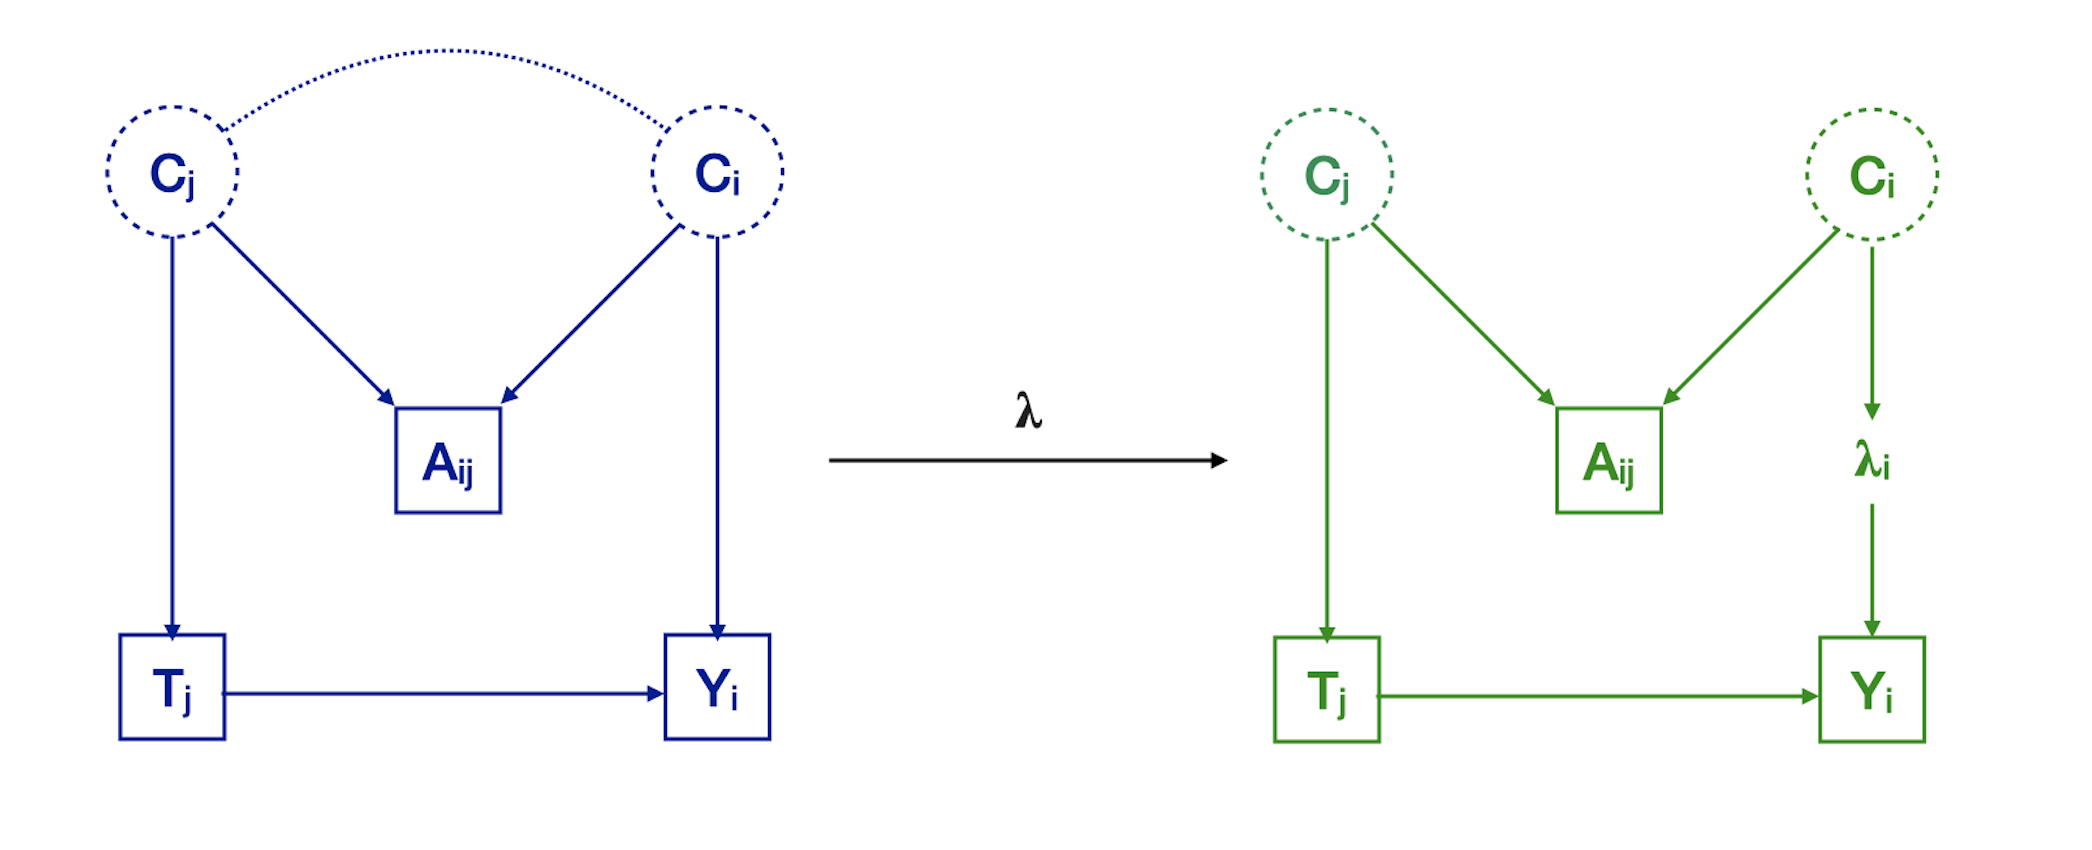
\includegraphics[width=\linewidth]{case1.png}
  \caption{Identification of causal effects using embeddings in a semi-supervised learning problem. This diagram shows a potential backdoor path passing through the unobserved confounders $C_j$ and $C_i$, while conditioning on the network structure (represented through the adjacency matrix variables $A_{ij}$) when attempting to estimate the effect of the treatment $T_j$ on the response $Y_i$. The figure shows that assuming $A_{ij}$ is conditionally independent from the response $Y_i$ given the embedding $\lambda_i$ and the treatment $T_i$ of node $i$ blocks problematic backdoor paths and allows for successful causal adjustment.}
  \label{fig:case1}
\end{figure}
\end{proof}


What if one seeks to perform causal adjustment on graphs in an unsupervised learning context? In such procedures, one would not have access to the unit labels anymore, thus assumption (i) of Theorem \ref{thm:identification} is no longer viable. One would however still have access to the proxy structure of the units, namely the matrix $A$, which would again induce a collider biases. 


\begin{cor} \textbf{Causal Identification via Embeddings in Unsupervised Learning Problems.}
\label{cor:identification}
Assume the set-up of Theorem \ref{thm:identification} and that the following conditions hold true:


\begin{itemize}
\item[i]  $A_{ij} \perp C  | \lambda_i, \mbox{ } \lambda_j$;
\item[ii]  Assumptions (i-iii) in Ogburn et al. (2020) \cite{Ogburn2020} described in Section \ref{sec:Ogburn};
\item[iii] $P(V = v| \lambda(c)) > 0, \mbox{ for all } v \mbox{ in the range of } V_i^*$, where $V_i^*$ is the summary function $V_i = s_{Y, i}(C_i, \{T_j: A_{ij} =1\})$ under the hypothetical intervention $ T = t^*$. 
\item[iv] $\lambda_i$ depends on $C_i$.  
\end{itemize}

Then, the same condition as that of Theorem \ref{thm:identification} holds true, that is, the causal parameter of interest $\mathbb{E}[\hat{Y}_n^*]$ is identified by

\begin{align}
\label{eqn:identification}
\psi = \frac{1}{n} \sum_{i=1}^n \mathbb{E}[m(V_i^*)] &= \frac{1}{n} \sum_{i=1}^n \sum_v m(v) h_{i, t^*} (v) \\
&= \frac{1}{n} \sum_{i=1}^n \sum_{c} m(s_{Y, i} (\lambda(c), t^*)) p_C(\lambda(c)),
\end{align}


\noindent where $m(s_{Y, i} (\lambda(c), t^*))$ and $p_C(\lambda(c))$ are the functions defined in Section \ref{sec:Ogburn}, representing quantities which can be estimated from the data.
\end{cor}


\begin{proof}
The ideas of the proof are analogous to those discussed in the proof of Theorem \ref{thm:identification}. We include diagram \ref{fig:case2} below which illustrates how conditioning on either of the embeddings $\lambda_i$ or $
\lambda_j$ blocks the backdoor paths between the variables $T_j$ and $Y_i$, and hence allows one to perform causal identification. 

\begin{figure}
  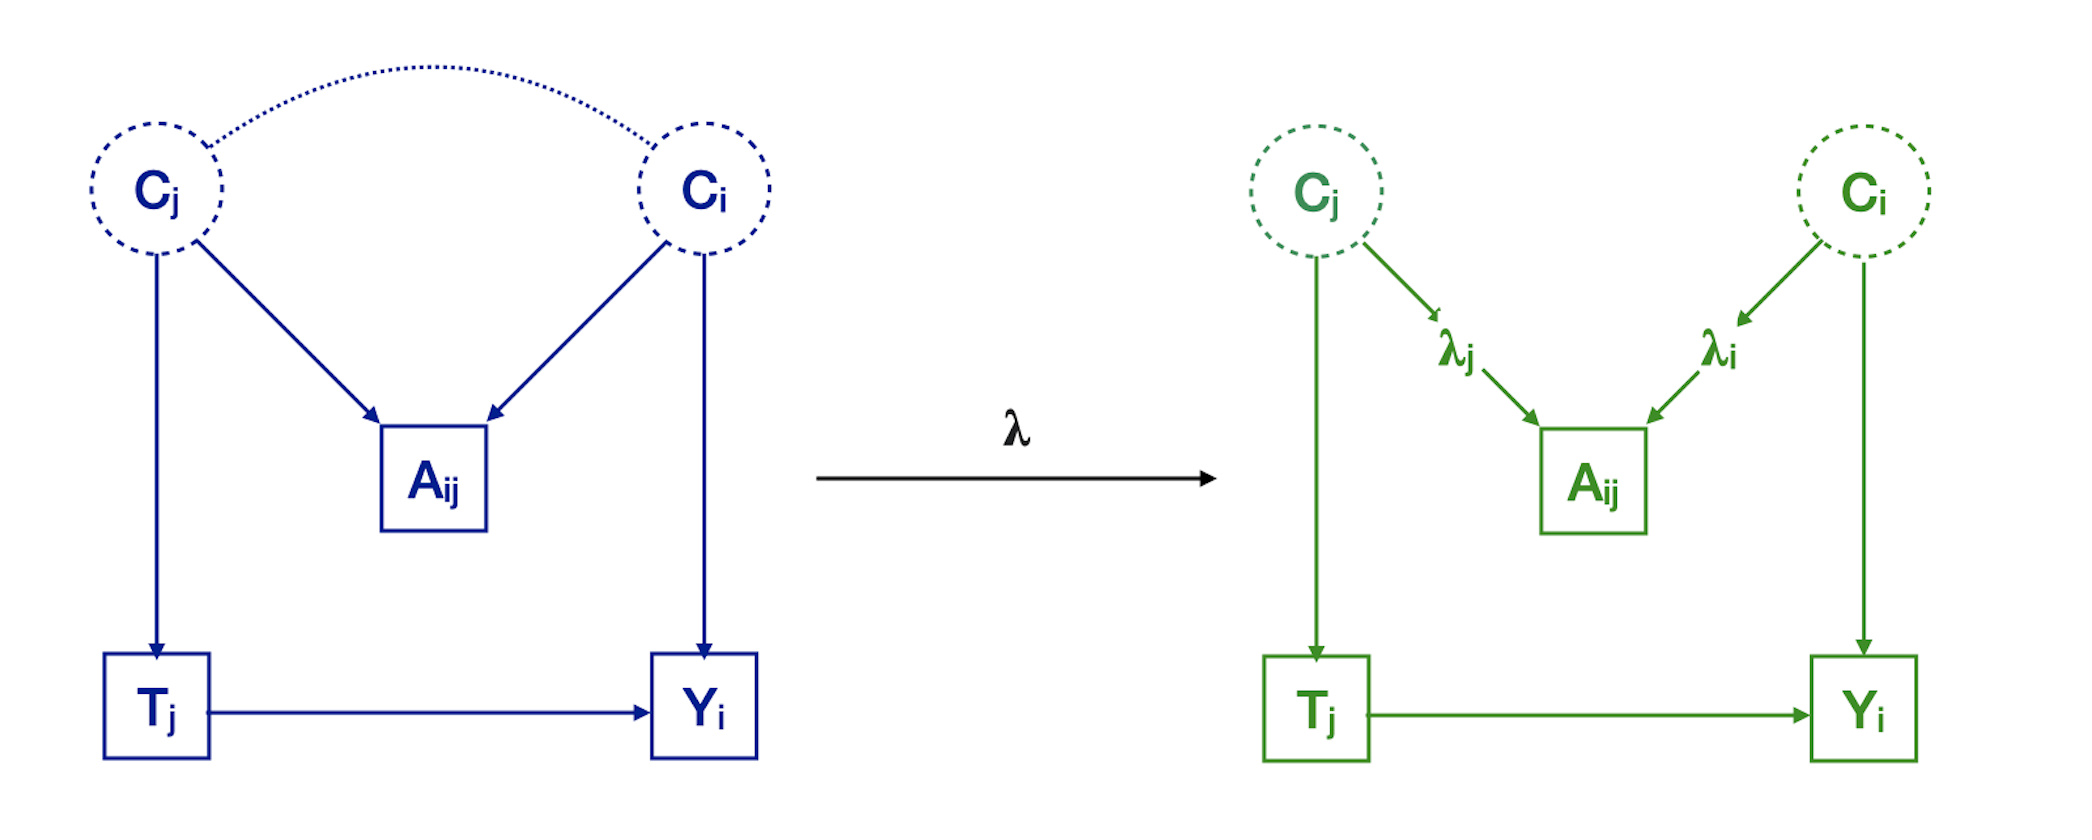
\includegraphics[width=\linewidth]{case2.png}
  \caption{Identification of causal effects using embeddings in a supervised learning problem. This diagram shows a potential backdoor path passing through the unobserved confounders $C_j$ and $C_i$, while conditioning on the network structure (represented through the adjacency matrix variables $A_{ij}$) when attempting to estimate the effect of the treatment $T_j$ on the response $Y_i$. The figure shows that assuming $A_{ij}$ is conditionally independent from the confounders $C_i$ and $C_j$ given the embeddings $\lambda_i$ and $\lambda_j$ of nodes $i$ and $j$, respectively, blocks problematic backdoor paths and allows for successful causal adjustment.}
  \label{fig:case2}
\end{figure}
\end{proof}

\textbf{Remark.} In both Theorem \ref{thm:identification} and Corollary \ref{cor:identification}, we expect condition (i) to hold true because embedding methods are tools which decouple the properties of the unit and the network structure, and have shown good empirical performance at explaining the local network structure (\cite{Hamilton:Ying:Leskovec:2018}). 

Having established how to identify causal effects using network embeddings, which could consist of \textit{any} established method, we now discuss how to estimate these effects from the data. 


\section{Estimation of Causal Effects}
\label{sec:estimation}
Recall that our causal parameter of interest $\mathbb{E}[\hat{Y}_n^*]$ was defined by equation \ref{eqn:identification} as

$$ \mathbb{E}[\hat{Y}_n^*] = \frac{1}{n} \sum_{i=1}^n \sum_{c} m(s_{Y, i} (\lambda_i(c), t^*)) p_C(\lambda_i(c)), $$


\noindent where $m(s_{Y, i}(\lambda_i(c), t^*)) = \sum_{y} u p_y(y|s_{Y, i}(\lambda_i(c), t^*))$ and $p_C(\lambda_i(c)) = p(\lambda_i(C) = \lambda_i(c))$ represent \textit{nuisance} parameters that we seek to estimate from the observed data and from the proxy (network structure) which carries information about the vector of unobserved covariates $\hat{C}$. Let $\eta_i = (m(s_{Y, i}(\lambda_i(c), t^*)), p_C(\lambda_i(c)))$ denote the pair of nuisance parameters for node $i$. 


Our goal is to obtain an estimate $\hat{\eta}$ of $\eta$ and then use it to compute an estimate $\hat{\psi}(O, \hat{\eta})$ of the causal parameter of interest $\psi$. In doing so, we seek to avoid using the same data $O = (Y, C, T)$ for both estimating the nuisance parameters and computing the causal estimate of interest, as this may affect the asymptotic properties of $\hat{psi}$. Thus, following the data splitting approach of \cite{Chernozhukov:Chetverikov:Demirer:Duflo:Hansen:Newey:2017}, we use one subset $I_0$ of the data to compute $\hat{\psi}$, and the rest of the data $I \backslash I_0$ to estimate $\eta$. 

We now describe how to obtain estimates of $m(s_{Y, i}(\lambda_i(c), t^*)$ and $p_C(\lambda_i(c)))$. We estimate $p_C(\lambda_i(c)))$ with the empirical distribution of the fitted embeddings. The estimation of $m(s_{Y, i}(\lambda_i(c), t^*)$ will however follow several steps, as outlined below. 

\noindent \textbf{Step 1.} We train a model using a relational empirical risk minimization procedure \cite{Veitch:Austern:Zhou:Blei:Orbanz:2019} in order to learn embeddings $\lambda_i$ such that $Y_i$ is estimated by $\mathbb{E}[Y_i| \lambda_i, s_{Y, i}(\{ T_j: A_{ij} =1\}) ]$ and such that $ q(\lambda_i)$ is a prediction for $s_{Y, i}(\{ T_j:A_{ij} =1\})$, given some function $q$. However, by simply noting that $s_{Y, i}(\{ T_j:A_{ij} =1\})$ is fully defined by $T_i$, it suffices to impose the condition that $q(\lambda_i, \gamma^T)$ is predictive of $T_i$. 

\smallskip

\noindent \textbf{Step 2.} We can then estimate $m(s_{Y, i}(\lambda_i(c), t^*)$ by 

$$ \hat{m}(t_i, \lambda_i, \gamma^m) = \mathbb{E}[Y_i | s(\{T_j|A_{ij}=1 \}), \lambda_i],$$

\noindent for each vertex. 

Let us give an example in order to illustrate the general approach of estimating the nuisance parameters. 

\noindent \textbf{Example.} Let Sample($G_n$, k) be a randomized sampling algorithm that returns a random subgraph of size $k$ from $G_n$, then define the following loss function

\begin{align*}
L(G_k, \lambda, \gamma^T, \gamma^m) &= \sum_{i \in I \ I_0} (y_i -  \hat{m}(t_i, \lambda_i, \gamma^m))^2 + \sum_{i \in I \ I_0} \mbox{CrossEntropy}(t_i, \hat{q}(\lambda_i, \gamma^T))   \\
 &+ \sum_{i, j \in I \times I} \mbox{CrossEntropy} (\mathbbm{1}[(i, j) \in G_k], \sigma(\lambda_i^T \lambda_j)).
\end{align*}

\noindent We then train

$$\hat{\lambda} \hat{\gamma}^T, \hat{\gamma}^m = \argmin_{\lambda, \gamma^T, \gamma^m} \mathbb{E}_{G_k = Sample(G_n, k)} [L(G_k, \lambda, \gamma^T, \gamma^m)]. $$


Having devised a method to estimate the nuisance parameters in the formula of the causal parameter of interest $\psi$, we are now ready to compute its estimate, by simply plugging in the values of the nuisance parameter estimates in equation \ref{eqn:identification}. As previously justified, for this step, we will be using the other part of the split data, namely the set $I_0$.

$$ \hat{\psi} = \frac{1}{|I_0|} \sum_{i=1}^{|I_0|} \sum_{c} \hat{m}(t_i, \lambda_i, \gamma^m) \hat{p}_C(\lambda(c)).$$

Having established how to obtain an estimator $\hat{\psi}$ of the average expected outcome of the responses $Y$, $\psi$, we next state an asymptotic normality result for this estimator, which will enable us to use normal approximations in finite samples, and construct 95\% confidence intervals around the estimated values $\hat{\psi}$. 



\section{Asymptotic Normality}

We establish an asymptotic result for the parameter of interest $\psi$, by considering a sequence of networks $\{G_n = (V_n, E_n)\}$ whose number of nodes goes to infinity ($\lim_{n \to \infty}|V_n| = \infty$), and such that the structural equation models specifying the distributions of the treatment, response, and covariates variables are preserved in the limit. 

For an arbitrary network $G$, let $K_i$ denote the degree of node $i$. Now, for a graph $G_n$ having $n$ nodes, let $K_{max, n} = \max_i{K_i}$ be the maximum degree of all its nodes. Our asymptotic result follows directly from that developed in \cite{Ogburn:Sofrygin:Diaz:vanderLaan:2017}. 

\begin{theorem}
Suppose that $K_{max, n}^2/n \to 0$, as $n  \to \infty$. Under assumptions (i)-(iii) from Section \ref{sec:Ogburn}, and assumption (iii) of Theorem \ref{thm:identification} (positivity assumption), for an arbitrary constant $C_n$ satisfying $n/K_{max, n}^2 \leq C_n \leq n$, we have 

$$\sqrt{C_n} (\hat{\psi} - \psi)  \xrightarrow[]{d} \mathcal{N}(0, \sigma^2), $$

\noindent where $\sigma^2$, the asymptotic variance of $\hat{\psi}$, is given by the variance of the influence curve of the estimator $\psi$. 
\end{theorem}


\begin{proof}
The proof follows by invoking Theorem 1 of \cite{Ogburn:Sofrygin:Diaz:vanderLaan:2017}. 
\end{proof}

\textbf{Remark.} It may seem stringent to assume that the maximum degree of the graph $G_n$,  $K_{max, n}$, has a growth rate of $O(\sqrt{n})$, given the fact that social networks typically exhibit the "small-world" property (\cite{Durrett:2006}), i.e. there exists a small number of highly influential nodes, which have very large degrees. However, this growth rate can controlled and diminished by further imposing a limit on the number of nodes that influence the few highly influential nodes. 


\printbibliography

\newpage
\appendix




\end{document}

